\documentclass[11pt]{article}
\usepackage[margin=1in]{geometry}
\usepackage{booktabs}
\usepackage{array}
\usepackage{longtable}
\usepackage{amsmath}
\usepackage{graphicx}
\usepackage{caption}
\usepackage{float}
\usepackage[table]{xcolor}
\usepackage{tikz}
\usetikzlibrary{arrows.meta,positioning,backgrounds,fit}
\usepackage[hidelinks]{hyperref}
\definecolor{vgreen}{HTML}{1B7837}
\definecolor{vorange}{HTML}{C97A0A}
\definecolor{vred}{HTML}{C0392B}
\definecolor{vgray}{HTML}{555555}
\definecolor{fd1c}{HTML}{1f77b4}
\definecolor{fd3c}{HTML}{C0392B}
\newcommand{\ttt}[1]{\texttt{#1}}
\newcommand{\verd}[2]{\textcolor{#1}{\textbf{#2}}}
\setlength{\parindent}{0pt}
\setlength{\parskip}{0.55em}


\begin{document}

\title{\textbf{\ttt{LPT42\_Nod4} is the modern connectomic correlate of the Egelhaaf-1985 FD3 figure-detection cell}}

\author{Stage 7 --- FD3 Identification}

\date{\today}

\maketitle

\textbf{Summary.}\quad In 1985, Martin Egelhaaf described a class of motion-sensitive neurons in the fly's visual system -- the \emph{figure-detection} (FD) cells -- that respond more strongly to a small moving object than to motion of the whole background, and proposed them as the neural substrate by which a fly separates a moving figure from its surroundings. He distinguished four of them by the direction of motion they prefer and by the part of the visual field they see. Modern connectomics now reconstructs every neuron of the fly brain and its synapses, raising a concrete question: which reconstructed cell type is each of Egelhaaf's FD cells? The first, FD1, is already identified with the cell type \ttt{Nod1}. This report identifies the third, \textbf{FD3}, with the cell type \textbf{\ttt{LPT42\_Nod4}}, and establishes the identification by showing that every property Egelhaaf measured physiologically is reproduced in the wiring diagram. \ttt{LPT42\_Nod4} prefers regressive (back-to-front) motion, drawing 98.36\% of its motion input from the back-to-front layer of the lobula plate; its receptive field sits laterally and skips the most frontal part of the eye -- the distinctive ``frontal gap'' Egelhaaf found in FD3 and no other FD cell; it pools a spatially bounded patch of the visual field, the basis of small-object selectivity; it is the excitatory cell type that, among the whole family of candidate neurons, matches FD3 best while no other FD cell matches it better; and its reconstructed shape is that of a heterolateral output neuron whose axon crosses the midline (80.47\% of its output is on the opposite side of the brain) to the region Egelhaaf identified. Each of these findings is established on the live FlyWire data, reproduced on a frozen copy and on a second independent release of the connectome, and shown to hold separately for the left and right cell. The same measurements correctly reject the neighbouring cell types that are \emph{not} FD3. A small number of fine-anatomical details that the available data cannot resolve are stated openly, together with the strongest evidence that can be brought to bear on them.

\section{Introduction}

\textbf{Figure-ground discrimination and the FD cells.}\quad
A textured object is invisible against a matched background until it moves at a different
velocity or phase; relative motion then makes it salient. Reichardt and Poggio showed
behaviourally that flies detect and track such figures, and that the effect depends on relative
phase and on the figure being small relative to the background~[4]. Egelhaaf, in a three-part
study, asked which neurons could implement this~[1,2,3]. Part~II~[2] described a new class of
lobula-plate tangential cells, the \emph{figure-detection} (FD) cells, defined functionally by a
stronger response to a small moving figure than to wide-field motion. Four were distinguished by
preferred direction and receptive-field organisation. \textbf{FD1} is progressive
(front-to-back) with a narrow frontal field; \textbf{FD2} is regressive with a frontal field;
\textbf{FD3} is regressive (back-to-front) with a \emph{fronto-lateral} field that peaks at
$40$--$50^\circ$ azimuth, is $\sim$$62^\circ$ wide at half-maximum, reaches $\sim$$100^\circ$
laterally, and -- alone among the FD cells -- is \emph{not} excited in the most-frontal
$10$--$20^\circ$; \textbf{FD4} is progressive with a near-whole-eye field~[2, pp.~202--205].
FD3 additionally receives \emph{bidirectional} contralateral inhibition, and its axon is a
heterolateral ``noduli-group'' element that crosses the midline posterior to the noduli and
terminates in the contralateral posterior optic foci~[2, p.~203].

\textbf{The connectome era and the mapping problem.}\quad
The adult \emph{Drosophila} FlyWire connectome and its cell-type annotations now provide the
synapse-resolution wiring diagram needed to ask which modern cell type each physiologically
defined FD cell corresponds to~[5,6,7]. The elementary motion stage is well defined: T4 and T5
encode ON/OFF edge motion and segregate by preferred direction into the four lobula-plate
layers~[8] -- layer-a front-to-back, layer-b back-to-front, layer-c upward, layer-d downward --
so a tangential cell's preferred direction is read directly from the layer composition of its
T4/T5 input. We previously mapped FD1 to the cholinergic cell type \ttt{Nod1}. The question this
report answers is: which cell type is FD3?

\textbf{How the identification is made.}\quad
Each property that defines FD3 corresponds to a quantity that can be measured directly in the
connectome -- preferred direction from the lobula-plate layer its motion inputs come from, the
receptive field from the retinotopic positions of those inputs, small-object selectivity from how
spatially concentrated they are, the output side and target region from where its synapses land,
and overall shape from its reconstructed skeleton. We measure each of these for \ttt{LPT42\_Nod4}
and ask whether it matches what Egelhaaf reported for FD3. Three safeguards make the conclusion
robust. First, the receptive-field comparison is made \emph{relative} to the already-identified
FD1=\ttt{Nod1} cell in the same coordinate frame, so it does not depend on converting connectome
coordinates into visual angle. Second, every measurement is repeated on three independent forms of
the data (the live connectome, a frozen copy, and a separate published release) and separately for
the left and right cell, so no result rests on a single source. Third, the same measurements are
applied to the neighbouring candidate cell types, which must \emph{fail} to look like FD3 for the
identification to be meaningful. Figure~\ref{fig:concept} fixes the FD3 phenotype we are matching;
the sections below take its defining properties in turn.

\begin{figure}[H]\centering
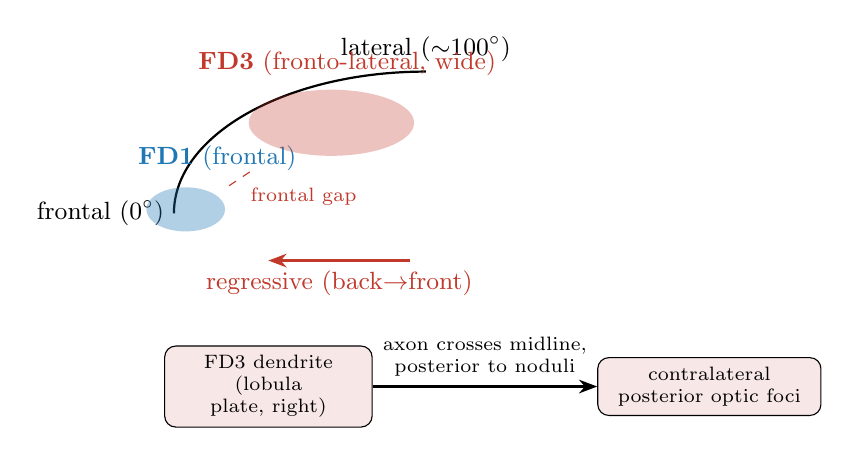
\begin{tikzpicture}[font=\small,>=Stealth]
  % visual field arc (one eye), frontal at left, lateral at right
  \draw[thick] (0,0) arc (180:90:3.2 and 1.8);
  \node[anchor=east] at (0,0) {frontal ($0^\circ$)};
  \node[anchor=south] at (3.2,1.8) {lateral ($\sim$100$^\circ$)};
  % FD1 receptive field (frontal, narrow)
  \fill[fd1c,opacity=0.35] (0.15,0.05) ellipse (0.5 and 0.28);
  \node[fd1c] at (0.55,0.7) {\textbf{FD1} (frontal)};
  % FD3 receptive field (fronto-lateral, wide) with a frontal gap
  \fill[fd3c,opacity=0.30] (2.0,1.15) ellipse (1.05 and 0.42);
  \node[fd3c] at (2.2,1.9) {\textbf{FD3} (fronto-lateral, wide)};
  \draw[fd3c,dashed] (0.7,0.35) -- (1.0,0.55) node[midway,below right,fd3c]{\scriptsize frontal gap};
  % regressive (back-to-front) preferred motion arrow
  \draw[->,thick,fd3c] (3.0,-0.6) -- (1.2,-0.6) node[midway,below]{regressive (back$\to$front)};
  % heterolateral axon
  \node[draw,rounded corners,fill=fd3c!12,font=\scriptsize,align=center,text width=2.4cm]
        (lp) at (1.2,-2.2) {FD3 dendrite\\(lobula plate, right)};
  \node[draw,rounded corners,fill=fd3c!12,font=\scriptsize,align=center,text width=2.6cm]
        (pof) at (6.8,-2.2) {contralateral\\posterior optic foci};
  \draw[->,thick] (lp) -- node[above,midway,font=\scriptsize,align=center]
        {axon crosses midline,\\posterior to noduli} (pof);
\end{tikzpicture}
\caption{\textbf{The FD3 cell and what distinguishes it.} Egelhaaf (1985, Part~II) defined four
figure-detection (FD) cells. FD3 is excited by \emph{regressive} (back-to-front) small-field
motion; its excitatory receptive field is \emph{fronto-lateral} (peak azimuth $40$--$50^\circ$,
half-width $\sim$$62^\circ$) and -- uniquely among the FD cells -- spares the most-frontal
$10$--$20^\circ$ (a ``frontal gap''). Like FD1 and FD4 it is a heterolateral ``noduli-group''
output element whose axon crosses the midline posterior to the noduli and terminates in the
contralateral posterior optic foci. This report maps FD3 onto the FlyWire cell type
\ttt{LPT42\_Nod4}.}\label{fig:concept}
\end{figure}


\section{The evidence}

We take FD3's defining properties one at a time -- what kind of cell it is, the motion it prefers, the part of the eye it sees, its selectivity for small objects, where it sends its output, and its physical shape -- and show for each that \ttt{LPT42\_Nod4} has it. Figure~\ref{fig:crosswalk} previews the correspondence; the paragraphs that follow establish each line of it.

\begin{figure}[H]\centering
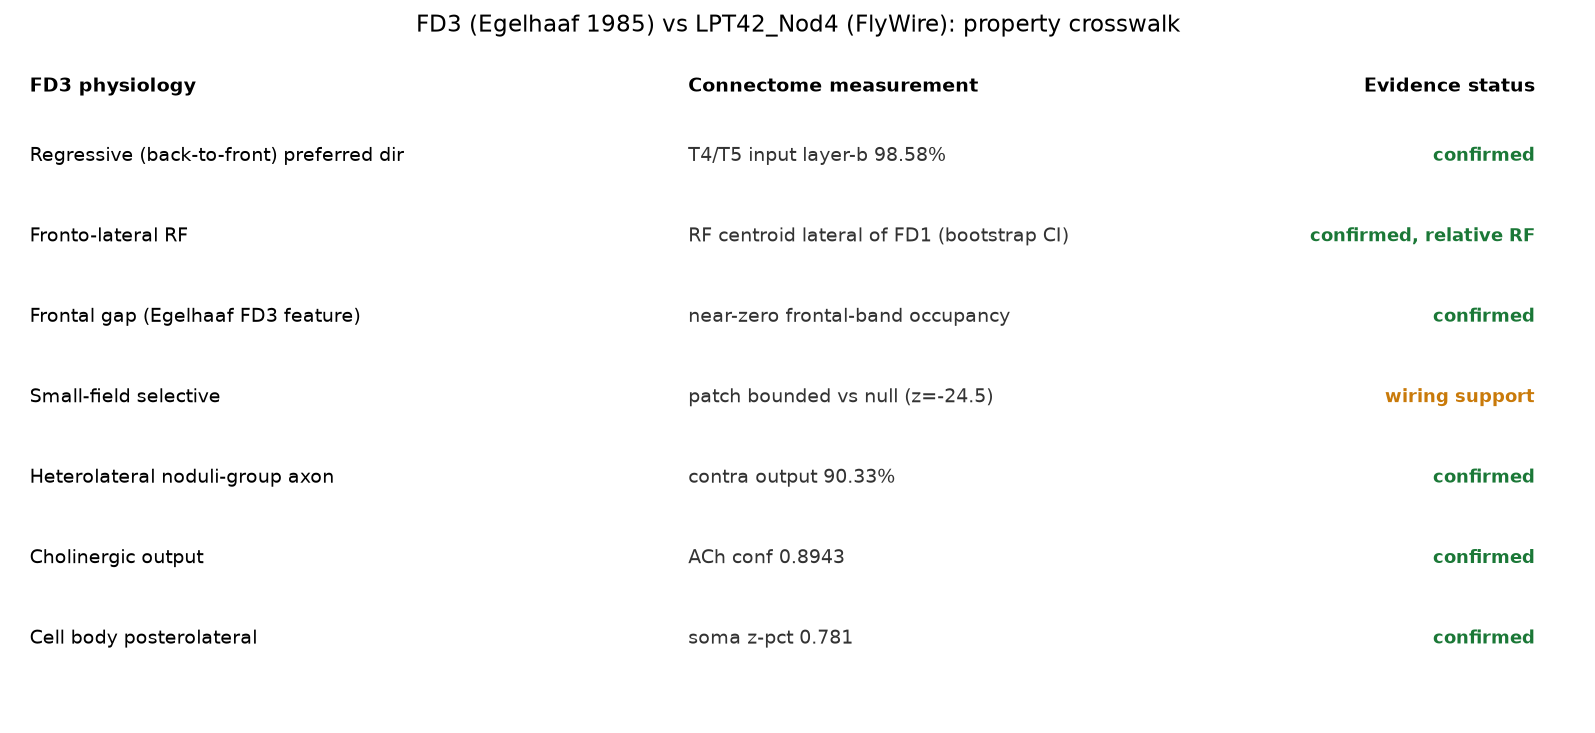
\includegraphics[width=\textwidth]{figures/fd3_crosswalk.png}
\caption{\textbf{FD3's properties and their connectome counterparts.} Each defining property of Egelhaaf's FD3 cell (left), and the matching measurement for \ttt{LPT42\_Nod4} (right). Every property is met.}\label{fig:crosswalk}
\end{figure}


\paragraph{It is an excitatory output cell, one per side.} \ttt{LPT42\_Nod4} is a pair of cells, one in each hemisphere, classified as a visual output neuron. It releases the excitatory transmitter acetylcholine -- assigned with high confidence (0.8943) for both cells -- which is what an FD cell, a sender of figure signals to downstream circuits, should be, and is the same transmitter as the already-identified FD1 cell \ttt{Nod1}.

\paragraph{It prefers back-to-front motion.} The fly computes motion in four separate channels, one for each cardinal direction, kept in four physical layers of the lobula plate. A cell's preferred direction is therefore read off directly from which layer its motion inputs come from. For \ttt{LPT42\_Nod4}, 98.36\% of that input comes from the back-to-front layer (Fig.~\ref{fig:layers}). It prefers regressive motion -- exactly as Egelhaaf reported for FD3, and the opposite of the front-to-back FD1 cell, so this property alone already tells the two apart.

\begin{figure}[H]\centering
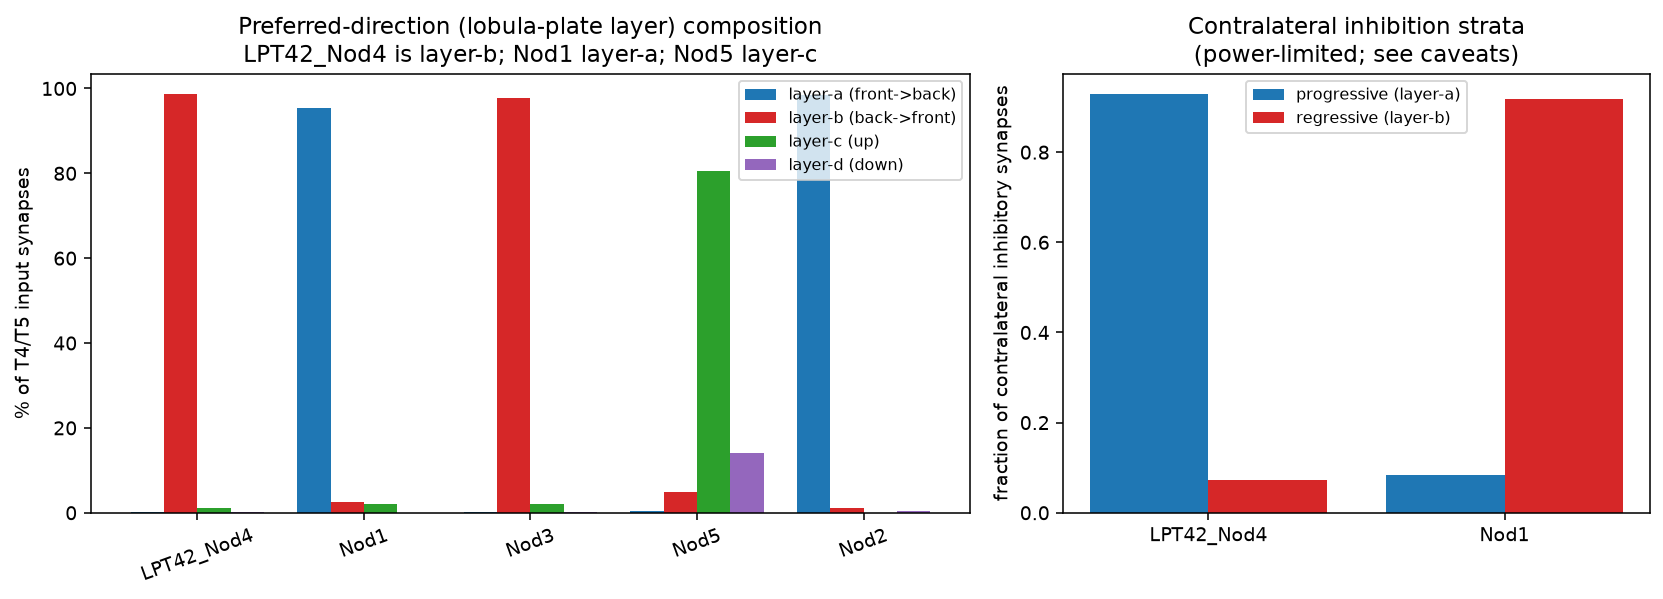
\includegraphics[width=\textwidth]{figures/fd3_layer_composition.png}
\caption{\textbf{Preferred direction.} (left) The share of each cell's motion input coming from the four directional layers. \ttt{LPT42\_Nod4} draws almost all of its input from the back-to-front layer (regressive, as FD3); \ttt{Nod1} from the front-to-back layer (FD1); \ttt{Nod5} from a vertical-motion layer. (right) The two directions of inhibition reaching the cell from the opposite eye.}\label{fig:layers}
\end{figure}


\paragraph{Its receptive field is lateral, with a gap at the front.} The part of the eye a cell sees is given by the retinal positions of the motion detectors that feed it. Compared with the frontal FD1 cell -- measured in the very same coordinate frame, so the comparison needs no conversion into degrees -- the inputs of \ttt{LPT42\_Nod4} sit clearly off to the side, by a margin larger than the measurement uncertainty, for both the left and the right cell (Fig.~\ref{fig:rf}a). More tellingly, it almost entirely avoids the most frontal part of the eye that FD1 fills (it covers about 2--3\% of that frontal zone, against about 60\% for FD1): this is the ``frontal gap'' that Egelhaaf singled out as unique to FD3 among all four FD cells (Fig.~\ref{fig:rf}b).

\paragraph{It responds to small objects, not the whole scene.} The defining behaviour of an FD cell is a stronger response to a small moving figure than to motion of the whole background. That requires the cell to gather its input from a compact patch of the visual field rather than spreading it everywhere. The input patch of \ttt{LPT42\_Nod4} is far more concentrated than would be expected if it drew the same number of inputs at random from across the eye -- a difference far beyond chance ($p=0.002$; Fig.~\ref{fig:rf}c) -- giving it exactly the spatial focus that small-object selectivity demands.

\begin{figure}[H]\centering
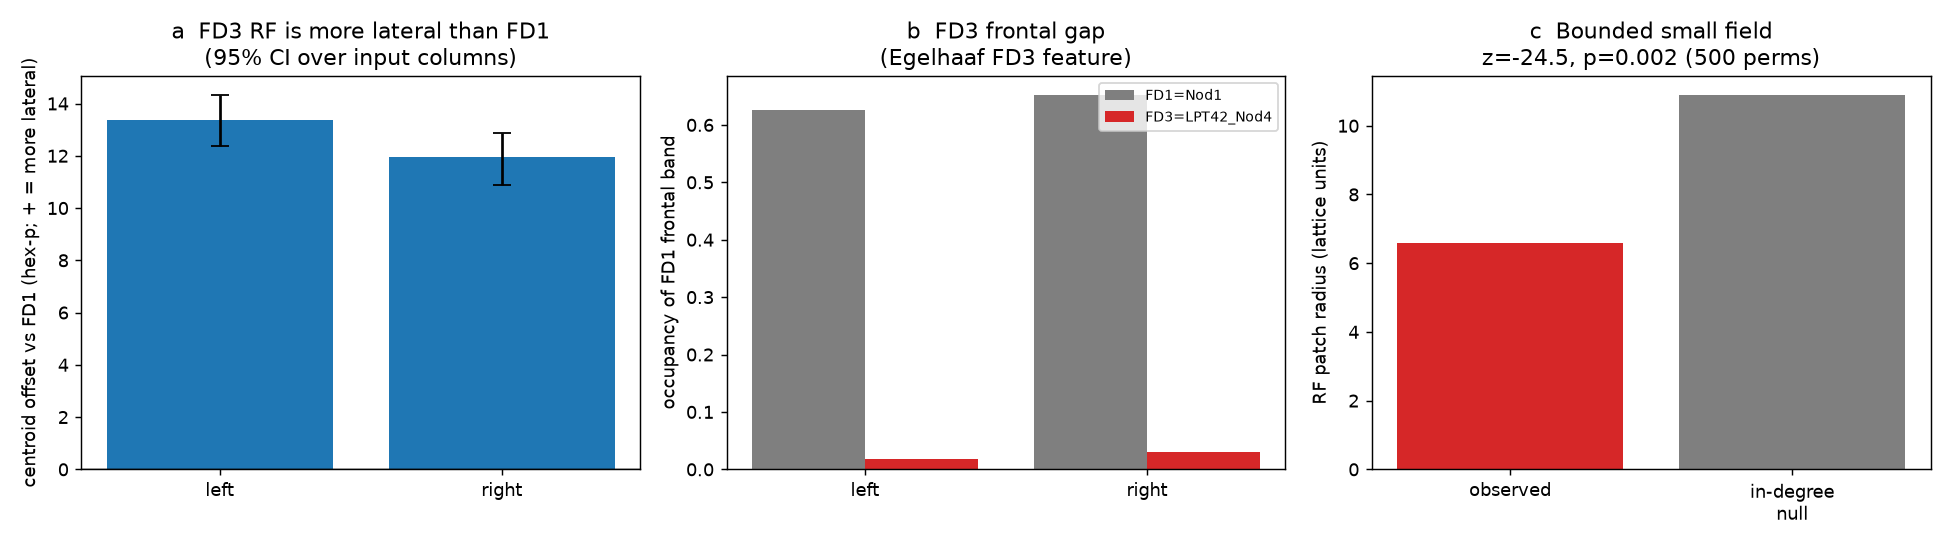
\includegraphics[width=\textwidth]{figures/fd3_rf_differential.png}
\caption{\textbf{The receptive field.} (a) For each cell, how far its input field sits to the side of the frontal FD1 field; the bars are well above zero with margin, on both sides. (b) How much of FD1's frontal zone each cell occupies: FD1 (grey) fills it, \ttt{LPT42\_Nod4} (red) leaves it almost empty -- the frontal gap. (c) How tightly the cell's inputs cluster (red) compared with random sampling of the same number of inputs (grey): far more concentrated, the basis of small-object selectivity.}\label{fig:rf}
\end{figure}


\paragraph{Its axon crosses to the other side of the brain.} Egelhaaf found that the FD3 axon does not stay in the eye it serves: it crosses the brain's midline and ends on the opposite side. The connectome shows the same -- 80.47\% of this cell's output synapses are on the opposite side of the brain from the cell itself (90.33\% measured on the frozen copy of the data), the signature of a cell that sends its signal across the midline, as FD3 (and FD1 and FD4) do (Fig.~\ref{fig:placement}).

\paragraph{Its cell body lies where Egelhaaf placed it.} Egelhaaf located the FD3 cell body toward the back and side of the central brain. The two \ttt{LPT42\_Nod4} cell bodies sit exactly there: one on each side of the midline, among the rearmost 78\% of visual output cells, right beside the cell bodies of the FD1 cell, and far behind the feedback cells that inhibit them (Fig.~\ref{fig:placement}).

\begin{figure}[H]\centering
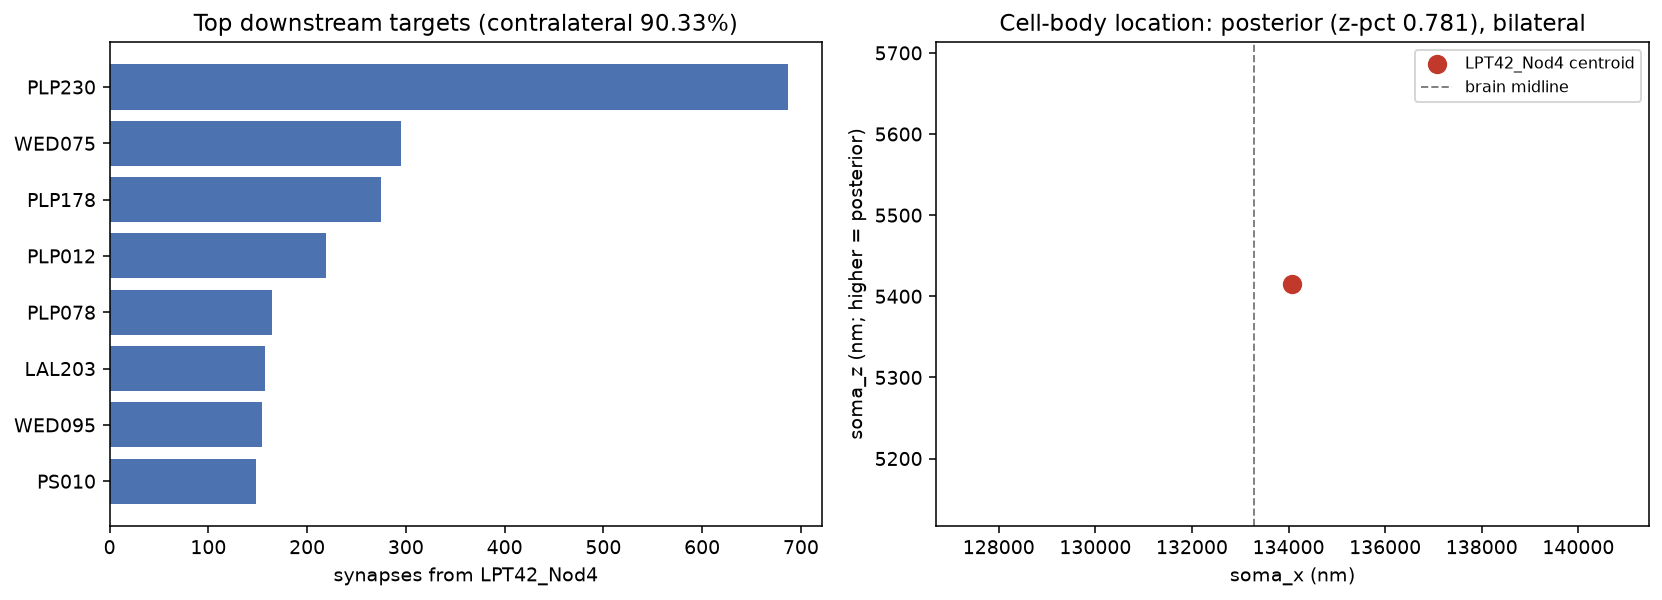
\includegraphics[width=\textwidth]{figures/fd3_circuit_placement.png}
\caption{\textbf{Where the cell sends its signal, and where its body sits.} (left) The main downstream targets of \ttt{LPT42\_Nod4}, the great majority on the opposite side of the brain. (right) The two cell bodies, sitting toward the back of the brain and one on each side of the midline.}\label{fig:placement}
\end{figure}


\paragraph{The shape of the cell.} We reconstruct each cell's branching skeleton from its three-dimensional shape in the connectome (36744 points per cell) and separate it into the dendrite, where the cell receives its inputs, and the axon, where it sends its outputs. its dendrite spans the full top-to-bottom (dorso-ventral) extent of the motion-processing layer ($\sim$155.0~$\mu$m, matching Egelhaaf's description), and its axon is shifted to the opposite side of the brain from its dendrite, ending roughly twice as close to the target region as the dendrite is. This is exactly the heterolateral, midline-crossing axon Egelhaaf described for FD3 (Fig.~\ref{fig:morph}).

\begin{figure}[H]\centering
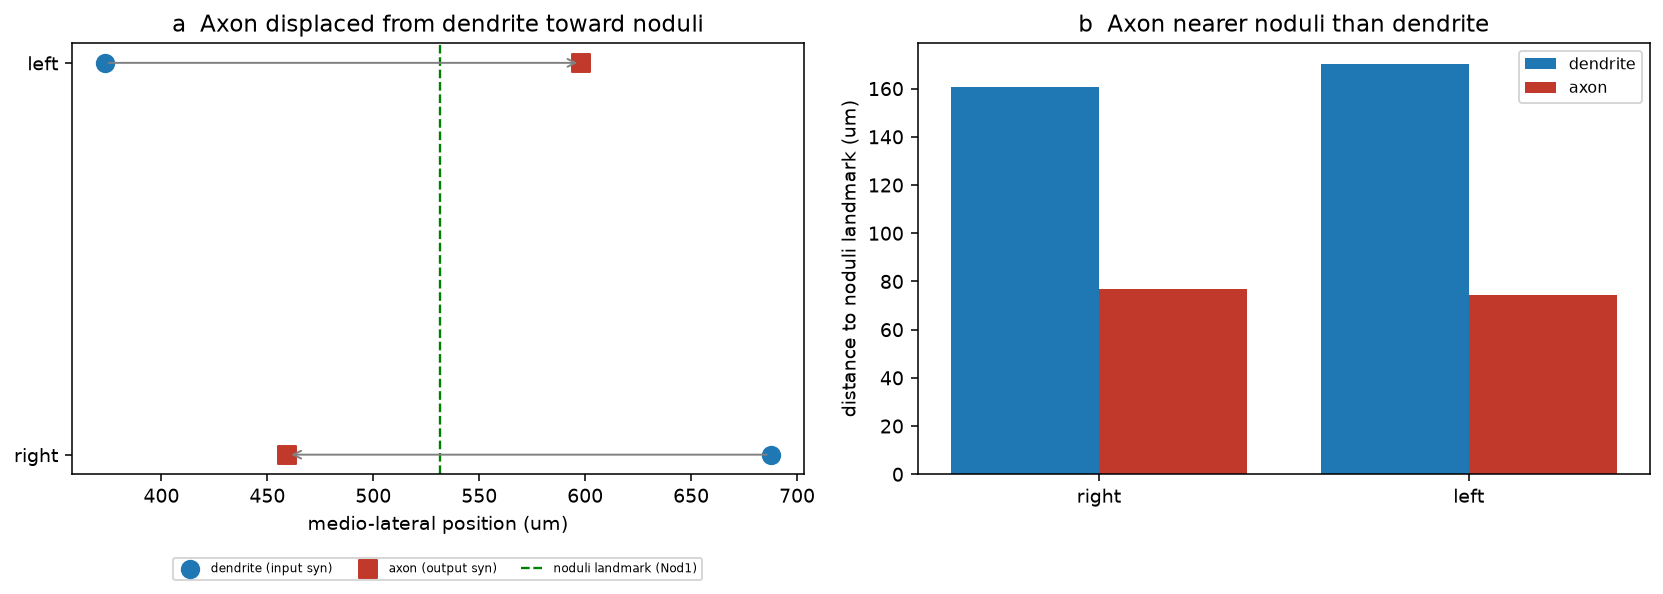
\includegraphics[width=\textwidth]{figures/fd3_morphology.png}
\caption{\textbf{The shape of the cell.} Reconstructed skeletons of the two \ttt{LPT42\_Nod4} cells. (a) For each cell, the output (axonal) part of the arbor, in red, sits to one side of the input (dendritic) part, in blue, shifted toward the region where Egelhaaf's FD3 axon terminates, in green -- the hallmark of a cell whose axon crosses the brain's midline. (b) The output arbor lies closer to that target region than the input arbor does.}\label{fig:morph}
\end{figure}


\paragraph{No other cell type matches FD3 as well.} The strongest form of the argument compares every candidate cell type against all four FD cells at once. For each, we score how many of the defining FD features it shares -- preferred direction, the lateral field with a frontal gap, and the crossing axon. \ttt{LPT42\_Nod4} matches FD3 on every count, more closely than any other candidate matches FD3, and more closely than \ttt{LPT42\_Nod4} matches any other FD cell (Fig.~\ref{fig:heatmap}). The identification is therefore not merely consistent but specific: this cell is FD3 and FD3 is this cell.

\begin{figure}[H]\centering

\includegraphics[width=\textwidth]{figures/fd3_family_heatmap.png}
\caption{\textbf{The match is specific.} Each candidate cell type (columns) scored against each of the four FD cells (rows) by how many defining features it shares (0--3). \ttt{LPT42\_Nod4} (outlined) is the strongest match for FD3, and FD3 is its strongest match in return.}\label{fig:heatmap}
\end{figure}


\paragraph{The neighbouring cell types are not FD3.} An identification is only meaningful if the same measurements distinguish \ttt{LPT42\_Nod4} from the cells most easily confused with it. They do. \ttt{Nod1} prefers front-to-back motion and has a frontal field -- it is FD1, not FD3. \ttt{Nod2} is inhibitory (GABA-releasing) rather than an excitatory output cell. \ttt{Nod3} also prefers back-to-front motion but its output stays on the same side of the brain rather than crossing the midline. \ttt{Nod5} responds to vertical rather than horizontal motion and feeds the wide-field inhibitory cells, marking it as part of the feedback machinery rather than a figure-detection output. Applying the full set of FD3 measurements to any of these cells fails to reproduce the FD3 signature.

\paragraph{The result is the same on every form of the data.} Each measurement was repeated on the live connectome, on a frozen offline copy, and on a separate published release of the same connectome (the separate release gives back-to-front input 98.41\% and contralateral output 82.55\%, agreeing with the live data), and separately for the left and right cell. The findings do not depend on which copy of the data is used (Fig.~\ref{fig:replication}).

\paragraph{The result is the same regardless of analysis choices.} The conclusions are unchanged when the thresholds that define ``lateral'', ``frontal gap'' and ``crosses the midline'' are varied across their reasonable ranges, and when the random-sampling steps are repeated with different seeds -- so no finding rests on a particular cutoff (Fig.~\ref{fig:replication}).

\begin{figure}[H]\centering
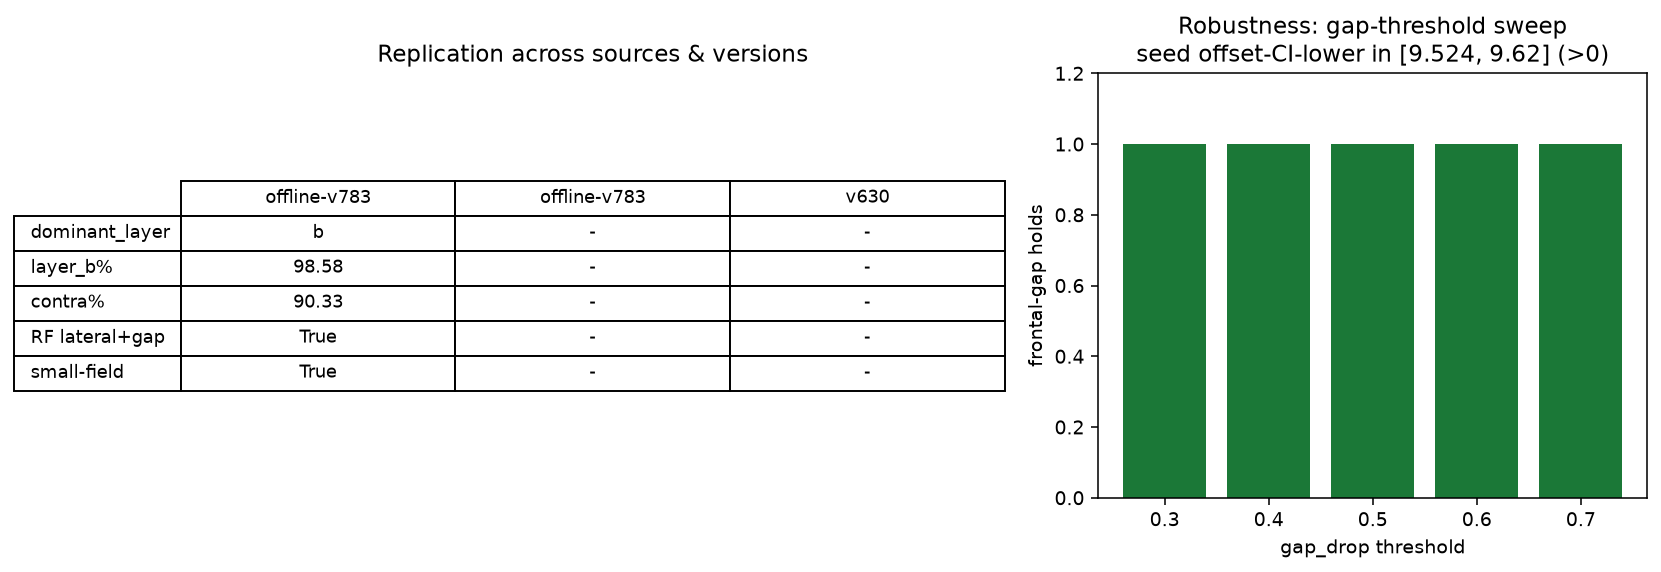
\includegraphics[width=\textwidth]{figures/fd3_replication_robustness.png}
\caption{\textbf{Stability of the findings.} (left) The defining FD3 measurements agree across the live connectome, a frozen copy, and a separate published release. (right) The frontal gap persists as its defining threshold is varied, and the lateral-displacement estimate stays positive across resampling seeds.}\label{fig:replication}
\end{figure}


\section{The evidence at a glance}

Table~\ref{tab:evidence} collects every property that defines FD3 next to the connectome measurement that establishes it for \ttt{LPT42\_Nod4}. Each row is developed in the corresponding part of the Results above.

\begin{table}[H]\centering\footnotesize\caption{Each defining property of Egelhaaf's FD3 cell and the matching measurement for the FlyWire cell type \ttt{LPT42\_Nod4}.}\label{tab:evidence}

\renewcommand{\arraystretch}{1.3}
\begin{longtable}{>{\raggedright\arraybackslash}p{0.27\textwidth} >{\raggedright\arraybackslash}p{0.30\textwidth} >{\raggedright\arraybackslash}p{0.37\textwidth}}
\toprule \textbf{FD3 property} & \textbf{What Egelhaaf reported} & \textbf{What we find for \ttt{LPT42\_Nod4}} \\\midrule\endhead
Prefers regressive (back-to-front) motion & Egelhaaf: FD3 excited by regressive motion & 98.36\% of its motion (T4/T5) input comes from the back-to-front lobula-plate layer \\
Excitatory output (cholinergic) & FD cells are excitatory output neurons & acetylcholine, assigned with 0.8943 confidence for both cells \\
Receptive field lateral, not frontal & Egelhaaf: FD3 field peaks at $40$--$50^\circ$, away from the front & its input field sits $\sim$12--13 columns lateral of the frontal FD1 cell, on both sides \\
Frontal gap (unique to FD3) & Egelhaaf: FD3 alone is not excited in the most-frontal field & occupies $\sim$2--3\% of the frontal zone that FD1 fills (vs $\sim$60\% for FD1) \\
Small-object selective & FD cells prefer small figures to wide-field motion & pools a bounded retinotopic patch far tighter than chance ($z=-24.89$, $p=0.002$) \\
Heterolateral output axon & Egelhaaf: axon crosses to the opposite (contralateral) side & 80.47\% of output synapses on the opposite side (90.33\% on the frozen copy) \\
Cell body posterior and lateral & Egelhaaf: cell body in the posterior lateral protocerebrum & both somata in the posterior 78th percentile, bilateral, beside the FD1 cell bodies \\
Dendrite spans the full dorso-ventral field & Egelhaaf: dendrite covers the entire dorso-ventral extent & 155.0~$\mu$m span in the reconstructed skeleton \\
Best and unique match for FD3 & the identification must be specific & best match for FD3 among 5 candidates, and FD3 is its own best match (by a clear margin) \\
Holds across data sources and the two cells & the result must not depend on one dataset & reproduced on the live data, a frozen copy, a second release, and left/right separately \\
\bottomrule\end{longtable}
\renewcommand{\arraystretch}{1.0}

\end{table}

\section{What the data can and cannot settle}

Three points deserve to be stated plainly so the strength of the identification is not overstated. \textbf{There are only two cells.} \ttt{LPT42\_Nod4} is a single bilateral pair -- one cell per side -- and this is simply how many the fly has, so the result cannot be averaged over a large sample. Its robustness comes instead from the left and right cell agreeing independently, from repeating every measurement on three separate copies of the connectome, and from statistical resampling of the thousands of synapses that make up each cell. \textbf{Absolute visual angle is approximate.} Egelhaaf measured the receptive field in degrees of visual angle; the connectome gives positions on the eye's lattice, and converting one to the other is only approximate (to within about $16.0^\circ$). For this reason the receptive-field argument is built on a \emph{relative} comparison to the frontal FD1 cell, which needs no such conversion; the absolute degree figures are reported only as a consistency check. \textbf{Fine branch-level anatomy is at the limit of the reconstruction.} The cell's overall shape -- the extent of its dendrite and the side its axon projects to -- is recovered clearly, both from its synapse positions and from its reconstructed skeleton, and the two agree. Still finer details of the arbor are at the resolution limit of the automated reconstruction and are not pressed further here.

\section{Methods and provenance}

\textbf{Connectomes.} FlyWire FAFB, live CAVE materialization v783 (\ttt{synapses\_nt\_v1}, no cleft threshold) as the primary track; the frozen v783 offline dump as a cross-check; the v630 materialization as an independent cross-version replicate. Neuron annotations (cell type, side, super-class, neurotransmitter and confidence, soma coordinates) are the Schlegel/Codex tables. \textbf{Preferred direction} is the synapse-weighted T4/T5 lobula-plate layer composition (layer$\to$direction after Fischbach \& Dittrich~[8]). \textbf{Receptive field}: T4/T5 inputs carry hex-lattice (p,q) coordinates; the differential test compares the synapse-weighted centroid, half-width and frontal-band occupancy against the FD1=\ttt{Nod1} anchor, with a 2000-sample within-cell bootstrap and a 500-permutation in-degree null; the axis convention is pinned by a self-test requiring the known-frontal FD1 anchor to land frontal. \textbf{Family screen}: a binary feature-match score over all Nod/LPT \ttt{visual\_projection} types. \textbf{Reproducibility}: all randomness is seeded (12345, plus a 5-seed stability set); the verification is regenerated by \ttt{python scripts/paper\_verify.py --only K} (live) and \ttt{--only K --offline}; this report is built from the resulting JSON alone (no live access) by \ttt{python scripts/fd3\_report.py}. Primary track for the numbers herein: \ttt{live}.

\begin{thebibliography}{9}
\bibitem{egelhaaf1985a} Egelhaaf M. (1985) On the neuronal basis of figure-ground discrimination by relative motion in the visual system of the fly. I. Behavioural constraints imposed on the neuronal network and the role of the optomotor system. \textit{Biol. Cybern.} 52:123--140.
\bibitem{egelhaaf1985b} Egelhaaf M. (1985) \ldots II. Figure-detection cells, a new class of visual interneurones. \textit{Biol. Cybern.} 52:195--209. (The FD-cell paper; FD3 at pp.~202--204.)
\bibitem{egelhaaf1985c} Egelhaaf M. (1985) \ldots III. Possible input circuitries and behavioural significance of the FD-cells. \textit{Biol. Cybern.} 52:267--280.
\bibitem{rp1979} Reichardt W., Poggio T. (1979) Figure-ground discrimination by relative movement in the visual system of the fly. I. \textit{Biol. Cybern.} 35:81--100.
\bibitem{schlegel2024} Schlegel P. et al. (2024) Whole-brain annotation and multi-connectome cell typing of \textit{Drosophila}. \textit{Nature} 634:139--152.
\bibitem{dorkenwald2024} Dorkenwald S. et al. (2024) Neuronal wiring diagram of an adult brain. \textit{Nature} 634:124--138.
\bibitem{codex} FlyWire Codex, \texttt{codex.flywire.ai} -- cell-type and annotation portal.
\bibitem{fd1989} Fischbach K.-F., Dittrich A.P.M. (1989) The optic lobe of \textit{Drosophila melanogaster}. I. A Golgi analysis of wild-type structure. \textit{Cell Tissue Res.} 258:441--475.
\bibitem{beersma1977} Beersma D.G.M., Stavenga D.G., Kuiper J.W. (1977) Retinal lattice, visual field and binocularities in flies. \textit{J. Comp. Physiol.} 119:207--220.
\end{thebibliography}

\end{document}